\documentclass[final,narroweqnarray,inline]{ieee}
% In order to use the figure-defining commands in ieeefig.sty...
\usepackage{ieeefig}
% To use utf8 encoding
\usepackage[utf8]{inputenc}
\begin{document}

%----------------------------------------------------------------------
% Title Information, Abstract and Keywords
%----------------------------------------------------------------------
\title[Trabajo Practico Nº 1: Wiretapping]{%
       Trabajo Practico Nº 1: Wiretapping}

% format author this way for journal articles.
\author[SHORT NAMES]{%
	Leandro Ezequiel Barrios,
	\and
	Gonzalo Benegas,
	\and
	Martin Caravario, 
	\and
	Pedro Rodriguez 
}

% make the title
\maketitle               

% do the abstract
\begin{abstract}
En el presente Trabajo Práctico utilizaremos algunas de las técnicas
provistas por la teoría de la información para estudiar y analizar algunas
redes de información. El objetivo será distinguir diversos aspectos de la
red de manera analítica. Para cumplir con nuestro objetivo, haremos uso de
dos herramientas modernas de manipulación y análisis de paquetes: Wireshark
y Scapy.
\end{abstract}

% start the main text ...


%
% Introducción
% Desarrollo Fuente S
%   Medicion Techint | Casa Marto | Casa Eze | Labos
% Desarrollo Fuente S_1
%   Medicion Techint | Casa Marto | Casa Eze | Labos
%----------------------------------------------------------------------
% SECTION I: Introduction
%----------------------------------------------------------------------
\section{ Introducción }

Construimos una herramienta que hace uso de la
función ``sniff'', provista por la librería Scapy de Python. Esta nos permitió escuchar durante
cierto tiempo la red local y guardarnos todos los paquetes que llegaban a
nuestra placa de red y eran levantados por esta. A partir de estos datos
que guardamos, fuimos capaces de encontrar  nodos y protocolos
distinguidos en la red a partir de la realización de gráficos de torta e histogramas apropiados.

Para cada una de las mediciones consideramos las siguientes fuentes: 
\begin{enumerate}
  \item $S = {s_{1} \dots s_{n}}$, provista por la cátedra, donde $s_{i}$ es el valor del campo
        \emph{type} del frame de capa 2. 
  \item $S_{1}$, elegida por nosotros, con la restricción de que todos los paquetes considerados
        debían ser de tipo ARP.
\end{enumerate}

ARP es un protocolo de la capa de enlace de datos, responsable de encontrar
la dirección de capa 2 (Ethernet MAC) que corresponde a una determinada
dirección IP (dirección de capa 3 de enlace). Es decir, cada vez que un host
quiere comunicarse con otro y su dirección MAC no se encuentra dentro de su
tabla ARP, debe enviar un paquete who-has broadcast para determinar la dirección MAC
del host destino. De este modo, todos los hosts del dominio de colisión de
esta máquina reciben dicho paquete, siendo respondido el mismo únicamente
por el host requerido, mediante un paquete rep, mediante un paquete reply.
Para distinguir nodos (símbolos) en este contexto, tomamos a aquellos cuya
probabilidad de aparición era alta, de forma tal que la información provista
por el mismo sea menor a la entropía de la fuente a la cuál el símbolo
pertenece.

\medskip
Para este ejercicio se decidi\'o tomar la siguiente fuente: \\ 
$S_{1}$ = \{$s_{1} \dots s_{n}$\} siendo el símbolo $s_{i}$ la tupla (src, dst), donde
src y dst son respectivamente las direcciones ip del emisor y receptor del
paquete ARP escuchado.  \\
Al analizar esta fuente, se busca identificar los nodos distinguidos. Es
decir, aquellos pares de ip que podemos concluir tienen mayor probabilidad de comunicarse
entre sí en la red escuchada, a partir de los datos obtenidos. 


\section{Experimentacion}


\subsection{Experimento 1}
Para este experimento se analiz\'o el trafico dentro de la red LAN de la empresa Techint, escuchando pasivamente
en la red durante media hora, con la herramienta desarrollada en el ejercicio 1. \\
Los resultados del experimento seran divididos segun la fuente utilizada (S o $S_{1}$), para poder analizar
entropias e informacion de sus respectivos simbolos de forma adecuada. \\
Los resultados obtenidos fueron los siguientes: 

\subsubsection{Fuente utilizada: S}

% \begin{figure}
% \begin{center}
%   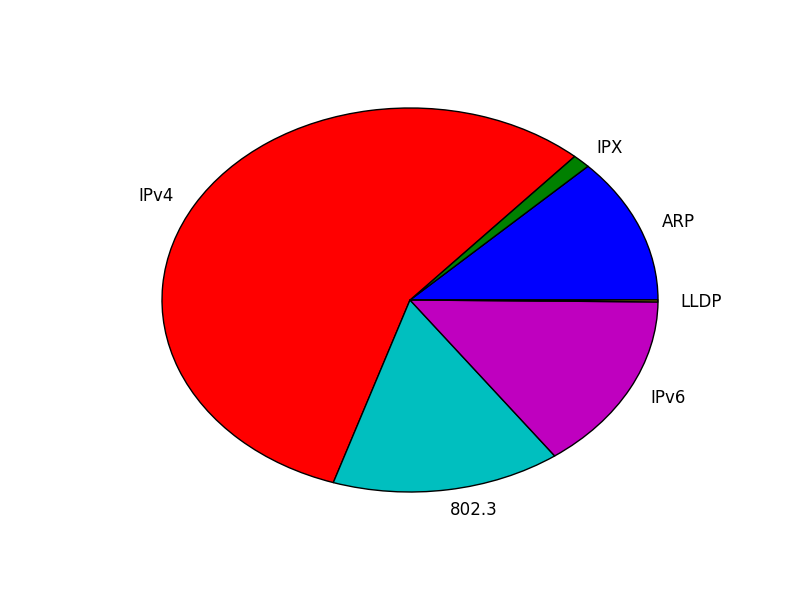
\includegraphics[width=0.5\textwidth]{graficos/techint-pie.png}
%   \caption{Techint - Gráfico torta}
%   \label{techint-pie}
% \end{center}
% \end{figure}

%\begin{figure}
%\begin{center}
%  \includegraphics[width=0.5\textwidth]{../output/labosdc-20150428-pie.png}
%  \caption{Labosdc20150428 - pie}
%  \label{labosdc20150428-pie}
%\end{center}
%\end{figure}

%{Grafico que muestra la proporción de cada protocolo dentro del total}
En este gráfico de torta se observa la cantidad de paquetes escuchados de cada
protocolo. Se pudieron escuchar protocolos de tipo IPv4, IPX, ARP, LLDP,
802.3 e IPv6. El símbolo mayormente emitido (con mayor probabilidad de
aparecer) por la fuente es IPv4.

%{Grafico que muestra la información que aporta cada protocolo y el corte de
%la entropía}
Este histograma muestra la cantidad de información provista por cada símbolo
de la fuente $S$ definida, calculada según la fórmula $ I(s_{i}) =
-log(p(s_{i}))  $. También hay un corte en la entropía de la fuente
(aproximadamente 1,9), que nos permite observar de manera sencilla cómo el símbolo (nodo)
distinguido de la fuente es IPv4.

\subsubsection{Fuente utilizada: $S_{1}$}

% do the biliography:
\bibliographystyle{IEEEbib}
\bibliography{my-bibliography-file}

% where ``my-bibliography-file.bib'' is the name of the file with all the 
% BibTeX entries.

% do the biographies...
%\begin{biography}{Gregory L. Plett}
%  A bio with no face...
%\end{biography}

% If you want a picture with your biography, then specify the name of
% the postscript file in square brackets. That is, uncomment the
% following three lines and change the name of "face.ps" to the name of 
% your file.
%\begin{biography}[face.ps]{Gregory L. Plett}
%  A bio with a face...
%\end{biography}

\end{document}
